\documentclass[oneside]{book}
\usepackage[svgnames]{xcolor}
\usepackage[british]{babel}
\usepackage[protrusion,expansion,babel,final]{microtype}
\usepackage[margin=1in]{geometry}
\usepackage[pdfversion=1.7]{hyperref}
\usepackage[shortlabels]{enumitem}
\usepackage{graphicx}
\usepackage{mathtools}
\usepackage{cleveref}
\usepackage{booktabs}
\usepackage{nicematrix}
\usepackage{derivative}
\usepackage{etoolbox}
\usepackage{siunitx}
\sisetup{round-mode = places, round-precision = 3, round-pad = false, retain-explicit-plus}
\usepackage{lmodern}
\usepackage[T1]{fontenc}
\usepackage[scaled=.98]{XCharter}
\usepackage[scaled=1.04,varqu,varl]{inconsolata}% inconsolata typewriter
\usepackage{amssymb}
\makeatletter
\@namedef{T1/zi4/m/it}{<->ssub*lmr/m/it}
\makeatother

\usepackage{bm}
\usepackage{tikz}
\usepackage{float}

% Functions
\providecommand\given{} % just to make sure it exists
\DeclarePairedDelimiterXPP{\E}[1]{\operatorname{\mathbb{E}}}[]{}{%
    \renewcommand\given{\nonscript\:\delimsize\vert\nonscript\:\mathopen{}}%
    \ifblank{#1}{\:\cdot\:}%
    #1}%
\DeclarePairedDelimiterXPP{\V}[1]{\operatorname{\textsf{V}}}(){}{%
    \renewcommand\given{\nonscript\:\delimsize\vert\nonscript\:\mathopen{}}%
    \ifblank{#1}{\:\cdot\:}%
    #1}%
\DeclarePairedDelimiterXPP{\Var}[1]{\operatorname{\textsf{Var}}}(){}{%
    \renewcommand\given{\nonscript\:\delimsize\vert\nonscript\:\mathopen{}}%
    \ifblank{#1}{\:\cdot\:}%
    #1}%
\DeclarePairedDelimiterXPP{\Cov}[1]{\operatorname{\textsf{Cov}}}(){}{%
    \renewcommand\given{\nonscript\:\delimsize\vert\nonscript\:\mathopen{}}%
    \ifblank{#1}{\:\cdot\:}%
    #1}%
\DeclarePairedDelimiterXPP{\Cor}[1]{\operatorname{\textsf{Cor}}}(){}{%
    \renewcommand\given{\nonscript\:\delimsize\vert\nonscript\:\mathopen{}}%
    \ifblank{#1}{\:\cdot\:}%
    #1}%
\DeclarePairedDelimiterXPP{\Covadj}[1]{\operatorname{\textsf{Cov}_{\text{adj}}}}(){}{%
    \renewcommand\given{\nonscript\:\delimsize\vert\nonscript\:\mathopen{}}%
    \ifblank{#1}{\:\cdot\:}%
    #1}%
\DeclarePairedDelimiterXPP\Prob[1]{\operatorname{\mathbb{P}}}(){}{%
    \renewcommand\given{\nonscript\:\delimsize\vert\nonscript\:\mathopen{}}%
    \ifblank{#1}{\:\cdot\:}%
    #1}%
\DeclarePairedDelimiterXPP\Ind[1]{\operatorname{\mathbb{I}}}\{\}{}{%
    \renewcommand\given{\nonscript\:\delimsize\vert\nonscript\:\mathopen{}}%
    \ifblank{#1}{\:\cdot\:}%
    #1}%
\DeclarePairedDelimiterXPP{\se}[1]{\operatorname{\textsf{se}}}(){}{%
    \ifblank{#1}{\:\cdot\:}%
    #1}%
\DeclarePairedDelimiterXPP{\seadj}[1]{\operatorname{\textsf{se}_{\text{adj}}}}(){}{%
    \renewcommand\given{\nonscript\:\delimsize\vert\nonscript\:\mathopen{}}%
    \ifblank{#1}{\:\cdot\:}%
    #1}%
\DeclarePairedDelimiterXPP{\estseadj}[1]{\operatorname{\widehat{\textsf{se}}_{\text{adj}}}}(){}{%
    \renewcommand\given{\nonscript\:\delimsize\vert\nonscript\:\mathopen{}}%
    \ifblank{#1}{\:\cdot\:}%
    #1}%
\DeclarePairedDelimiterXPP{\estse}[1]{\widehat{\operatorname{\textsf{se}}}}(){}{%
    \ifblank{#1}{\:\cdot\:}%
    #1}%
\DeclarePairedDelimiterXPP{\estV}[1]{\widehat{\operatorname{\textsf{V}}}}(){}{
    \renewcommand\given{\nonscript\:\delimsize\vert\nonscript\:\mathopen{}}%
    \ifblank{#1}{\:\cdot\:}%
    #1}%
\DeclarePairedDelimiterXPP{\estVar}[1]{\widehat{\operatorname{\textsf{Var}}}}(){}{
    \renewcommand\given{\nonscript\:\delimsize\vert\nonscript\:\mathopen{}}%
    \ifblank{#1}{\:\cdot\:}%
    #1}%
\let\exp\relax%
\let\log\relax%
\let\ln\relax%
\DeclarePairedDelimiterXPP{\exp}[1]{\operatorname{\textsf{exp}}}\{\}{}{#1}%
\DeclarePairedDelimiterXPP{\log}[1]{\operatorname{\textsf{log}}}(){}{#1}%
\DeclarePairedDelimiterXPP{\ln}[1]{\operatorname{\textsf{ln}}}(){}{#1}%
\DeclarePairedDelimiterXPP{\diag}[1]{\operatorname{\textsf{diag}}}(){}{#1}%
\DeclarePairedDelimiterXPP{\sign}[1]{\operatorname{\textsf{sign}}}(){}{#1}%

\DeclarePairedDelimiterXPP{\expit}[1]{\operatorname{\textsf{expit}}}(){}{#1}%
\DeclarePairedDelimiterXPP{\logit}[1]{\operatorname{\textsf{logit}}}(){}{#1}%
\newcommand{\HN}{\textsl{H}_{\textsl{0}}}%
\newcommand{\HA}{\textsl{H}_{\textsl{A}}}%

% Distributions
\DeclarePairedDelimiterXPP{\N}[1]{\mathcal{N}}(){}{#1}%
\DeclarePairedDelimiterXPP{\POI}[1]{\text{POI}}(){}{#1}%
\DeclarePairedDelimiterXPP{\BIN}[1]{\text{BIN}}(){}{#1}%
\DeclarePairedDelimiterXPP{\BERN}[1]{\text{BERN}}(){}{#1}%
\DeclarePairedDelimiterXPP{\MVN}[1]{\text{MVN}}(){}{#1}%
\DeclarePairedDelimiterXPP{\NB}[1]{\text{NB}}(){}{#1}%
\DeclarePairedDelimiterXPP{\GAM}[1]{\text{GAM}}(){}{#1}%
\DeclarePairedDelimiterXPP{\BetaDist}[1]{\text{Beta}}(){}{#1}%

\newcommand{\iid}{\overset{\text{iid}}{\sim}}%
\newcommand{\ind}{\overset{\text{ind}}{\sim}}%
\newcommand{\OR}{\text{OR}}%
\newcommand{\RR}{\text{RR}}%
\newcommand{\cOR}{\text{cOR}}%

\DeclarePairedDelimiter\abs{\lvert}{\rvert}
% can be useful to refer to this outside \Set
\newcommand\SetSymbol[1][]{%
    \nonscript\:#1\vert{}
    \allowbreak\nonscript\:
    \mathopen{}}
\DeclarePairedDelimiterX\Set[1]\{\}{%
    \renewcommand\given{:}
    #1
}
\DeclareMathOperator*{\argmax}{arg\,max}
\DeclareMathOperator*{\argmin}{arg\,min}
\DeclareMathOperator*{\arginf}{arg\,inf}
\DeclareMathOperator*{\argsup}{arg\,sup}

\providecommand{\RandomVector}[1]{\bm{#1}}% general vectors in bold italic
\providecommand{\Vector}[1]{\bm{#1}}% general vectors in bold italic
\providecommand{\Matrix}[1]{\bm{#1}}
\providecommand{\MatrixCal}[1]{\bm{\mathcal{#1}}}
\providecommand{\Field}[1]{\bm{#1}}

\usepackage{stackengine}
\usepackage[british]{isodate}
\newcommand{\makeheading}[2]%
{%
\begin{center}%
    \makebox[\linewidth]{\raisebox{-.5ex}[0cm][0cm]{\stackanchor{\textcolor{Gray}{\textsc{#1}}}{\scriptsize\itshape\printyearoff#2}\;}\color{Crimson!50}\hrulefill}%
\end{center}%
}%

\usepackage[breakable]{tcolorbox}
\tcbset{
    regular/.style={
        boxrule=0pt,
        breakable,
        sharp corners
    }
}

\newtcolorbox{Example}[1]{regular,colframe=Green!20!white,colback=Green!10!white,coltitle=Green,title={#1}}%
\newtcolorbox{Regular}[1]{regular,colframe=Navy!15!white,colback=Navy!5!white,coltitle=Navy,title={#1}}%
\newtcolorbox{Result}[1]{regular,colframe=Red!15!white,colback=Red!5!white,coltitle=Red,title={#1}}%

\hypersetup{colorlinks=true,%
linkcolor=[rgb]{0,0.5,1},%
pdftitle={Statistical Methods for Life History Analysis (STAT 437)},%
pdfauthor={Cameron Roopnarine, Dylan Spicker},%
pdfsubject={Statistics},%
pdfkeywords={University of Waterloo, Winter 2022 (1221)}}%

\title{%
\LARGE Statistical Methods for Life History Analysis\\%
\large STAT 437\\%
\normalsize Winter 2022 (1221)\thanks{Online Course}}%
\author{Cameron Roopnarine\thanks{\LaTeX{}er}\and Dylan Spicker\thanks{Instructor}}%
\date{\today}%
\usepackage{pgfplots}
\pgfplotsset{compat=1.18}
\usetikzlibrary{petri,decorations.pathreplacing,calc}
\usepackage{framed}

\begin{document}
\maketitle
\tableofcontents
\chapter{What are Longitudinal Data?}
\makeheading{Week 1}{\daterange{2022-01-05}{2022-01-07}}%chktex 8
\section{What are Longitudinal Data?}
\begin{figure}[H]
    \centering
    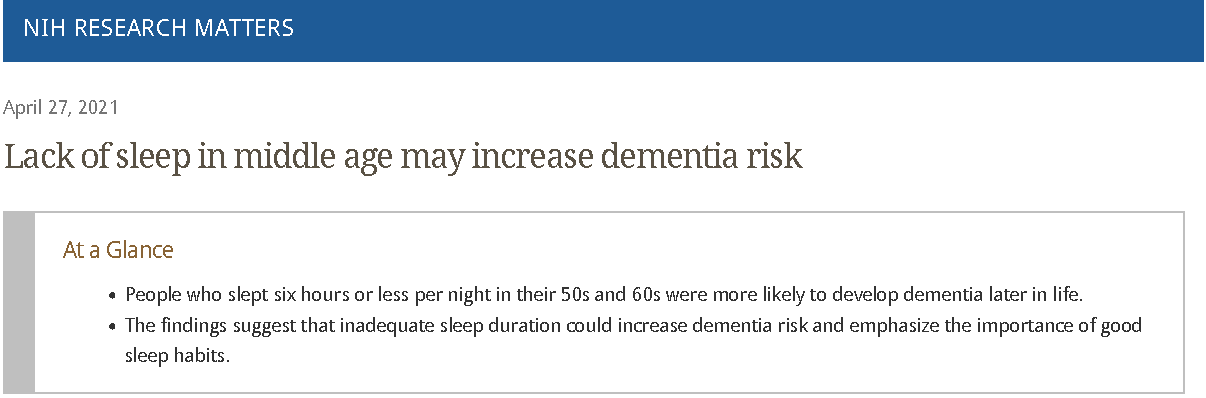
\includegraphics[width=\textwidth]{figures/002-study.pdf}
\end{figure}
What would a study \textbf{need} to look like to conclude this?
\subsection{The Design of a Longitudinal Study}
\begin{itemize}
    \item Can we conclude this by taking a sample of elderly individuals directly?
          \begin{itemize}
              \item \textbf{No}. How do we determine how much they slept 20 years prior?
          \end{itemize}
    \item Can we conclude this by taking a sample of middle-aged individuals directly?
          \begin{itemize}
              \item \textbf{No}. How do we determine who will develop dementia later on?
          \end{itemize}
    \item Can we conclude this by taking independent samples of middle-aged individuals \emph{and}
          elderly individuals?
          \begin{itemize}
              \item \textbf{No}. How do we pair the individuals?
          \end{itemize}
\end{itemize}
We would \emph{need} to be able to follow individuals, starting when they are middle-aged,
recording information like how often they sleep, and continue following them until the
onset of dementia.
\begin{framed}
    \centering\textbf{This is a longitudinal study}.
\end{framed}
\begin{figure}[H]
    \centering
    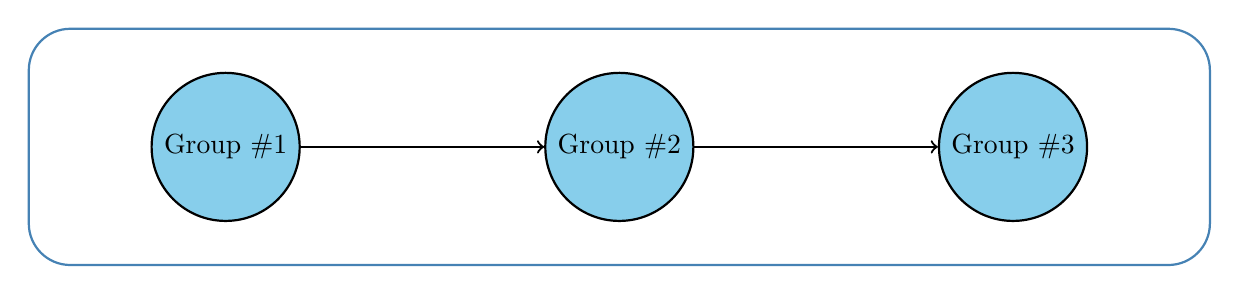
\begin{tikzpicture}[thick]
        \draw[rounded corners=15pt,SteelBlue] (10,0) rectangle ++(15,3);
        \node[draw,circle,fill=SkyBlue] (A) at (12.5,1.5) {Group \#1};
        \node[draw,circle,fill=SkyBlue] (B) at (17.5,1.5) {Group \#2};
        \node[draw,circle,fill=SkyBlue] (C) at (22.5,1.5) {Group \#3};
        \draw[->] (A) -- (B);
        \draw[->] (B) -- (C);
    \end{tikzpicture}
    \caption{Longitudinal Study}
\end{figure}
\begin{figure}[H]
    \centering
    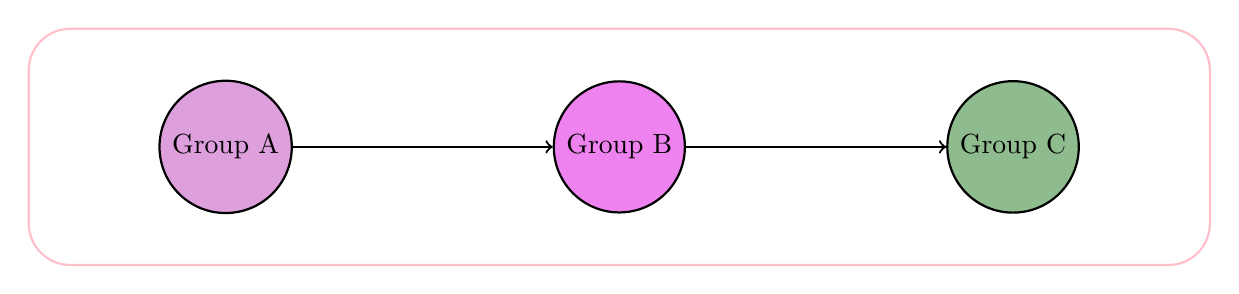
\begin{tikzpicture}[thick]
        \draw[rounded corners=15pt,Pink] (10,0) rectangle ++(15,3);
        \node[draw,circle,fill=Plum] (A) at (12.5,1.5) {Group A};
        \node[draw,circle,fill=Violet] (B) at (17.5,1.5) {Group B};
        \node[draw,circle,fill=DarkSeaGreen] (C) at (22.5,1.5) {Group C};
        \draw[->] (A) -- (B);
        \draw[->] (B) -- (C);
    \end{tikzpicture}
    \caption{Cross-Sectional Study}
\end{figure}
A research study in which \textbf{subjects are followed over time}.
Typically, this involves
repeated measurements of the same variables.
Longitudinal studies differ from \textbf{cross-sectional} studies and
\textbf{time series} studies.
\subsection{Uses for Longitudinal Studies}
\begin{itemize}
    \item To detect \emph{changes} in outcomes, both at the population and individual level.
    \item \textbf{Longitudinal effects} as compared to \textbf{cohort effects}.
    \item Correctly ascertain the exposures.
    \item Understand different sources of variation
    \item \textbf{Between}- and \textbf{within}-subject variation.
    \item To detect \textbf{time effects}, both directly and as interactions with other relevant
          factors.
\end{itemize}
Bottom line: There are many questions of interest which can only be answered using
longitudinal data. We should probably learn how to analyse it.
\subsection{Why are Longitudinal Data Special?}
What makes longitudinal data more difficult to analyse?
\begin{itemize}
    \item The data are \textbf{correlated}.
    \item Everyone's favourite assumption
          (assume that $ X_1,\ldots,X_n $ are iid) will \textbf{not} hold.
    \item Now what? STAT 437.
\end{itemize}
\subsection{Example Datasets}
\subsubsection{TLC Trial}
\begin{table}[H]
    \centering
    \begin{tabular}{cccccc}
        \toprule
        ID     & Treatment & W0     & W1     & W4     & W6     \\
        \midrule
        1      & P         & 30.8   & 26.9   & 25.8   & 23.8   \\
        2      & A         & 26.5   & 14.8   & 19.5   & 21     \\
        3      & A         & 25.8   & 23     & 19.1   & 23.2   \\
        \vdots & \vdots    & \vdots & \vdots & \vdots & \vdots \\
        98     & A         & 29.4   & 22.1   & 25.3   & 4.1    \\
        99     & A         & 21.9   & 7.6    & 10.8   & 13     \\
        100    & A         & 20.7   & 8.1    & 25.7   & 12.3   \\
        \bottomrule
    \end{tabular}
\end{table}
\begin{itemize}
    \item Is there a difference between \textbf{placebo} and \textbf{treatment}?
    \item How does the blood lead level \textbf{change over time} (in each group)?
    \item Is the \textbf{change} over time \textbf{equal} between treatment groups?
\end{itemize}
\subsubsection{Sales Data}
\begin{table}[H]
    \centering
    \begin{tabular}{ccccc}
        \toprule
        \texttt{DATE} & \texttt{brand} & \texttt{prod} & \texttt{QTY} & \texttt{PROMO} \\
        \midrule
        2014-01-02    & 1              & 1             & 7            & 0              \\%chktex 8
        2014-01-02    & 1              & 2             & 3            & 0              \\%chktex 8
        2014-01-02    & 1              & 3             & 0            & 0              \\%chktex 8
        \vdots        & \vdots         & \vdots        & \vdots       & \vdots         \\%chktex 8
        2018-12-31    & 4              & 8             & 1            & 1              \\%chktex 8
        2018-12-31    & 4              & 9             & 0            & 0              \\%chktex 8
        2018-12-31    & 4              & 10            & 3            & 1              \\%chktex 8
        \bottomrule
    \end{tabular}
\end{table}
\begin{itemize}
    \item Are the \textbf{different brands comparable} in terms of overall sales?
    \item Are the \textbf{different products comparable}?
    \item Do \textbf{promotions increase} the quantity sold? If so, \textbf{by how much}?
    \item Do the effects of time, and promotion, \textbf{change by brand} or product?
\end{itemize}
\subsubsection{Podcast Data}
\begin{table}[H]
    \centering
    \begin{tabular}{ccccc}
        \toprule
        Rating & No. Reviews & Title                  & Date       & $\cdots$ \\
        \midrule
        4.9    & 6400        & Dissect                & 2019-11-01 & $\cdots$ \\%chktex 8
        4.9    & 26300       & The Adventure Zone     & 2019-11-01 & $\cdots$ \\%chktex 8
        4.8    & 3700        & Song Exploder          & 2019-11-01 & $\cdots$ \\%chktex 8
        \vdots & \vdots      & \vdots                 & \vdots     & \vdots   \\%chktex 8
        4.2    & 1100        & Finding Fred           & 2019-12-01 & $\cdots$ \\%chktex 8
        3.9    & 648         & Inside Frozen 2        & 2019-12-01 & $\cdots$ \\%chktex 8
        4.6    & 6400        & Pop Culture Happy Hour & 2019-12-01 & $\cdots$ \\%chktex 8
        \bottomrule
    \end{tabular}
\end{table}
\begin{itemize}
    \item Can we \textbf{predict} the number of ratings that a podcast will receive over time?
    \item Can we \textbf{predict} the average rating value that a podcast will receive over time?
\end{itemize}
\subsubsection{Stroke Data}
\[ \begin{array}{ccccc}
        \toprule
        \texttt{year} & \text{Prop.}~(0,0) & \text{Prop.}~(0,1) & \text{Prop.}~(1,0) & \text{Prop.}~(1,1) \\
        \midrule
        1             & 57 / 344           & 17 / 72            & 17 / 79            & 5 / 23             \\
        2             & 27 / 287           & 8 / 55             & 9 / 62             & 4 / 18             \\
        3             & 23 / 260           & 8 / 47             & 5 / 53             & 3 / 14             \\
        \vdots        & \vdots             & \vdots             & \vdots             & \vdots             \\
        8             & 10 / 129           & 1 / 15             & 5 / 23             & 1 / 4              \\
        9             & 17 / 119           & 3 / 14             & 4 / 18             & 0 / 3              \\
        10            & 13 / 102           & 1 / 11             & 2 / 14             & 0 / 3              \\
        \bottomrule
    \end{array} \]
\begin{itemize}
    \item $0 =$ placebo treatment, $1 =$ active treatment; $0 =$ no previous stroke, $1 =$ previous stroke.
    \item This is \textbf{time to event} data.
    \item What is \textbf{probability of surviving} beyond some point?
    \item Does this \textbf{differ} if you previously had a stroke? If you \textbf{received treatment}?
\end{itemize}
\subsection{Summary}
\begin{itemize}
    \item Longitudinal data occur when we take repeated measurements on the same
          individuals over time.
    \item Longitudinal data are required for answering questions about changes within an
          individual (compared to between individuals) and to capture time effects.
    \item Longitudinal data are challenging to work with because the data are correlated.
\end{itemize}
\section{Exploring Longitudinal Data (Application)}
R Demo.
%<<child='003.Rnw'>>=
%@
\section{Notation for Longitudinal Data (Theory)}
\subsection*{General Notation}
\begin{itemize}
      \item Random variables: $ X $, $ Y $, $ Z $.
            \begin{itemize}
                  \item Realizations of these random variables: $ x $, $ y $, $ z $.
            \end{itemize}
      \item Unknown parameters:
            $ \theta $, $ \beta $, $ \alpha $.
            \begin{itemize}
                  \item Estimates of these parameters with ``hat:''
                        $ \hat{\theta} $, $ \hat{\beta} $, $ \hat{\alpha} $.
            \end{itemize}
      \item Transpose of a matrix $ \Matrix{X} $: $ \Matrix{X}^\top $.
\end{itemize}
\subsection*{Individual Notation}
\begin{itemize}
      \item Individual outcome for individual
            $ i $ at time $ j $: $ Y_{ij} $, where $ i=1,\ldots,n $
            are the individuals, and $ j=1,\ldots,k_i $ are the time points.
            We may also use $ Y_{it_j} $ to denote the outcome
            for individual $ i $ at time $ t_j $ when more complex times are used.
      \item Individual variate: $ X_{ijk} $, where $ i $ and $ j $
            index over individuals and times, respectively, and $ k $ indexes over the
            different variates of interest.
            \begin{Example}{}
                  Suppose for an individual that
                  we measure age, treatment, and symptom status.
                  We have $ k=3 $ since we have three variables.
            \end{Example}
      \item Usually, $ X_{ijk} $ will not change over time,
            so we may write $ X_{ijk}=X_{ij^\prime k} $ for all $ j $
            and $ j^\prime $. Usually $ X_{ij1}=1 $ to include the intercept
            in our models. However, if a variate is time-changing, then
            we need to be more careful about $ X_{ij1}=1 $.
      \item For an individual, define
            $\Matrix{Y}_i=\begin{bmatrix}
                        Y_{i1} \\
                        Y_{i2} \\
                        \vdots \\
                        Y_{ik_i}
                  \end{bmatrix}_{\mathrlap{k_i\times 1}}\equiv
                  (Y_{i1},Y_{i2},\ldots,Y_{ik_i})^\top$
            to be a vector of outcomes.
      \item For variates, take $ \Matrix{X}_{ij}=\begin{bmatrix}
                        X_{ij1} &
                        X_{ij2} &
                        \cdots  &
                        X_{ijp}
                  \end{bmatrix}_{1\times p}\equiv(X_{ij1},X_{ij2},\ldots,X_{ijp}) $,
            where $ p $ different variates are measured.
      \item Define
            $\Matrix{X}_i=\begin{bmatrix}
                        \Matrix{X}_{i1} \\
                        \Matrix{X}_{i2} \\
                        \vdots          \\
                        \Matrix{X}_{ik_i}
                  \end{bmatrix}_{\mathrlap{p\times k_i}}$
            to be a matrix containing of all the variates.
      \item In certain contexts, we may write $ \Matrix{Y}_i $
            as a row vector or to take the transpose of $ \Matrix{X}_i $.
\end{itemize}
\subsection{Notation and Considerations for Time}
\begin{itemize}
      \item Time for the $ i\textsuperscript{th} $
            individual at the $ j\textsuperscript{th} $ measurement: $ t_{ij} $.
            \begin{itemize}
                  \item Sometimes, we take $ t_{ij}=j $, where $ j $ is an index of visits.
                  \item If the scale of time is related to calendar time,
                        we may have $ t_{i1}=0 $ and $ t_{i2}=14 $ to indicate the first visit and second
                        visit are two weeks apart, where time is measured in days.
            \end{itemize}
      \item The design is \textbf{balanced} if $ t_{ij}=t_{i^\prime j} $
            for all $ i $ and $ i^\prime $. In this case,
            we drop subscript $ i $ from the times and write $ t_1,\ldots,t_k $.
            We will often consider balanced designs, but this is not necessary.
\end{itemize}
\section{What is Linear Regression (Review/Theory)}
\subsection*{The Ordinary Least Squares Estimators}
\begin{itemize}
    \item Suppose $ \Matrix{Y}_i $ are continuous, and we want to model $ \E{\Matrix{Y}_i\given \Matrix{X}_i} $.
    \item A \textbf{linear regression model} takes
          \[ \E{\Matrix{Y}_i\given \Matrix{X}_i}=\Matrix{X}_i\Vector{\beta}. \]
    \item We take
          \[ \hat{\Vector{\beta}}=(\Matrix{X}^\top \Matrix{X})^{-1}\Matrix{X}^\top\Matrix{Y}, \]
          and we call these \textbf{ordinary least squares} (OLS) estimators.
\end{itemize}
\subsection*{OLS Estimators (Two Ways)}
\begin{itemize}
    \item If $ \Matrix{Y}_i\mid \Matrix{X}_i \sim \N{\Matrix{X}_i \Matrix{\beta},\sigma^2} $,
          then the OLS estimators are the \textbf{maximum likelihood estimators}.
    \item If we take $ \Matrix{Y}_i=\Matrix{X}_i \Matrix{\beta}+\Matrix{\varepsilon}_i $,
          where $ \Matrix{\varepsilon}_i $ is non-normal, then the OLS estimators
          are simply the best (in terms of \emph{mean squared error})
          predictor of $ \Matrix{\beta} $.
\end{itemize}
\subsection*{Assumptions for OLS}
\begin{enumerate}[1.]
    \item The conditional mean is \textbf{linear} (in parameters).
    \item All values of $ \Matrix{Y}_i $ have constant variance,
          denoted $ \sigma^2 $ (conditionally).
    \item The $ \Matrix{Y}_i $ are \textbf{independent}.
\end{enumerate}
\subsection*{Asymptotic Analysis}
\begin{itemize}
    \item As $ n\to \infty $, $ \hat{\Vector{\beta}}\sim\N[\big]{\Matrix{\beta},\Var{\hat{\Vector{\beta}}}} $,
          where
          \[ \Var{\hat{\Vector{\beta}}}=\sigma^2(\Matrix{X}^\top \Matrix{X})^{-1}. \]
          We can use this result for \textbf{confidence intervals}
          and \textbf{hypothesis tests}.
\end{itemize}
\subsection*{Summary}
\begin{itemize}
    \item Linear Regression allows us to estimate a functional form for the conditional mean
          of a continuous outcome.
    \item The OLS estimators are valid MLE-type estimators when normality is assumed, and
          are LS estimators otherwise.
    \item The asymptotic analysis is valid in large samples, regardless of distributional
          assumptions, and can be used for Wald-type analysis.
\end{itemize}
\section{Why Can't We Just Use Regression? (Linear Marginal Models)}
\subsection*{Stated Mathematically}
We want to \textbf{fit a model} that gives
$ \E{Y_{ij}\given \Matrix{X}_{ij},t_{ij}} $
in terms of \textbf{interpretable parameters}.
\subsection*{Let's use an example!}
\[ \begin{array}{cccccccccc}
        \toprule
        \texttt{ID} & \texttt{Trt} & \texttt{W0} & \texttt{W1} & \texttt{W4} & \texttt{W6} & \texttt{ID} & \texttt{Trt} & \texttt{time} & W      \\
        \midrule
        1           & \texttt{P}   & 30.8        & 26.9        & 25.8        & 23.8        & 1           & \texttt{P}   & 1             & 30.8   \\
        2           & \texttt{A}   & 26.5        & 14.8        & 19.5        & 21          & 2           & \texttt{A}   & 1             & 26.5   \\
        3           & \texttt{A}   & 25.8        & 23          & 19.1        & 23.2        & 3           & \texttt{A}   & 1             & 25.8   \\
        \vdots      & \vdots       & \vdots      & \vdots      & \vdots      & \vdots      & \vdots      & \vdots       & \vdots        & \vdots \\
        98          & \texttt{A}   & 29.4        & 22.1        & 25.3        & 4.1         & 98          & \texttt{A}   & 4             & 4.1    \\
        99          & \texttt{A}   & 21.9        & 7.6         & 10.8        & 13          & 99          & \texttt{A}   & 4             & 13     \\
        100         & \texttt{A}   & 20.7        & 8.1         & 25.7        & 12.3        & 100         & \texttt{A}   & 4             & 12.3   \\
        \bottomrule
    \end{array} \]
\begin{itemize}
    \item Consider the TLC trial data, in \textbf{wide format} (left-hand side) and then in \textbf{long
              format} (right-hand side).
    \item In the right-hand side we have an outcome ($W$), with two explanatory factors
          \big($ \Set{\texttt{Trt},\texttt{time}} $\big).
          \begin{itemize}
              \item We want $ \E{W\given \texttt{Trt},\texttt{time}} $. \textbf{Is this familiar}?
          \end{itemize}
\end{itemize}
\subsection*{Using Linear Regression}
We can fit the model in R, using \texttt{lm}. \textbf{Is this valid}?
\[ \begin{tabular}{l
            S[table-format=-2.3]
            S[table-format=2.3]
            S[table-format=0.3]}
        \toprule
                                  & {Estimate} & {Std. Error} & {$\Prob{>\abs{t}}$} \\
        \midrule
        \texttt{(Intercept)}      & 26.540     & 0.9370175    & 0.0000000           \\
        \texttt{time2}            & -13.018    & 1.3251428    & 0.0000000           \\
        \texttt{time3}            & -11.026    & 1.3251428    & 0.0000000           \\
        \texttt{time4}            & -5.778     & 1.3251428    & 0.0000166           \\
        \texttt{TreatmentP}       & -0.268     & 1.3251428    & 0.8398322           \\
        \texttt{time2:TreatmentP} & 11.406     & 1.8740349    & 0.0000000           \\
        \texttt{time3:TreatmentP} & 8.824      & 1.8740349    & 0.0000035           \\
        \texttt{time4:TreatmentP} & 3.152      & 1.8740349    & 0.0933783           \\
        \bottomrule
    \end{tabular} \]
\subsection*{What does this \texttt{lm} imply about our data?}
\begin{itemize}
    \item There is a \textbf{linear conditional mean structure}:
          \begin{align*}
              \E{W_{ij}\given \texttt{Trt}_i,t_j}
               & =\beta_0+\beta_1\texttt{Trt}_i+\beta_2\Ind{t_j=2}+\beta_3\Ind{t_j=3}+\beta_4\Ind{t_j=4} \\
               & \quad+\beta_5\texttt{Trt}_i\Ind{t_j=2}
              +\beta_6\texttt{Trt}_i\Ind{t_j=3}+\beta_7\texttt{Trt}_i\Ind{t_j=4}.
          \end{align*}
    \item There is \textbf{constant variance} such as $ \Var{W_{ij}}=\sigma^2 $
          for all $ i $ and $ j $.
    \item The values of $ W_{ij} $ are \textbf{independent}. However,
          this assumption is clearly violated.
\end{itemize}
\subsection*{What makes longitudinal data special?}
Longitudinal data are characterized by \textbf{correlation} \emph{within} individuals.

TODO figure
Therefore, the previous \texttt{lm} will work \textbf{only if} we are willing
to assume that the observations are
\textbf{independent}.
\subsection*{Longitudinal Data as Multivariate Data}
How can we adapt linear regression to allow for this
association?
\begin{itemize}
    \item When the data are in \textbf{long format}, it appears that the outcomes are univariate.
    \item When the data are in \textbf{wide format}, we can view the outcome as a vector of
          outcomes, (e.g., $ \Matrix{W}=(W_0,W_1,W_4,W_6) $).
    \item The analysis of longitudinal data is \textbf{multivariate analysis}.
          \begin{itemize}
              \item This accounts for the \textbf{lack of independence} in the outcomes!
          \end{itemize}
\end{itemize}
\subsection*{Multivariate Normal}
Instead of assuming that $ Y_{ij}\sim \N{\Matrix{X}_{ij}\beta,\sigma^2} $,
what if we took
\[ \Matrix{Y}_i \sim \MVN{\Matrix{X}_i\Matrix{\beta},\Matrix{\Sigma}_i}? \]
\textbf{Recall}: The multivariate normal (MVN) has a density given by
\[ f(\Matrix{y},\Matrix{\mu},\Matrix{\Sigma})=
    \frac{1}{(2\pi)^{k/2}}\abs{\Matrix{\Sigma}}^{-1/2}
    \exp*{-\frac{1}{2}(\Matrix{y}-\Matrix{\mu})\Matrix{\Sigma}^{-1}(\Matrix{y}-\Matrix{\mu})^\top}.
\]
\subsection*{Linear Marginal Models}
\begin{itemize}
    \item In this proposal, we specify a \textbf{linear form} for the conditional mean.
          \begin{itemize}
              \item That is, $ \E{\Matrix{Y}_i\given \Matrix{X}_i}=\Matrix{X}_i \Matrix{\beta} $,
                    where $ \Matrix{X}_i $ is a matrix and $ \Matrix{Y}_i $ is a vector.
          \end{itemize}
    \item We allow for \textbf{correlation} through the individual covariance
          matrix, $ \Matrix{\Sigma}_i $.
    \item We could (theoretically) find the \textbf{MLE} under the assumption of
          multivariate normality.
\end{itemize}
\subsection*{Covariance Matrix}
Recall that $ \Cor{X,Y}=\frac{\Cov{X,Y}}{\sqrt{\Var{X}\Var{Y}}} $,
and so, re-arranging,
\[ \Cov{X,Y}=\Cor{X,Y}\sqrt{\Var{X}\Var{Y}}.\]
Moreover, recall that a variance/covariance matrix is
\[ \Cov{\Matrix{Y}_i}=
    \Matrix{\Sigma}_i=
    \begin{bmatrix}
        \Var{Y_{i1}}        & \Cov{Y_{i1},Y_{i2}} & \cdots & \Cov{Y_{i1},Y_{ip}} \\
        \Cov{Y_{i2},Y_{i1}} & \Var{Y_{i2}}        & \cdots & \Cov{Y_{i2},Y_{ip}} \\
        \vdots              & \vdots              & \ddots & \vdots              \\
        \Cov{Y_{ip},Y_{i1}} & \Cov{Y_{ip},Y_{i1}} & \cdots & \Var{Y_{ip}}
    \end{bmatrix}. \]
\subsection*{Covariance Matrix Simplification}
If \textbf{we assume} that $ \Var{Y_{ij}}=\sigma^2 $
for all $ i, j $, \emph{and} we denote $ \Cor{Y_{ij},Y_{i\ell}}=\rho_{j\ell} $
for all $ i $, then note that
\[ \Cov{Y_{ij},Y_{i\ell}}=\Cor{Y_{ij},Y_{i\ell}}\sqrt{\Var{Y_{ij}\Var{Y_{i\ell}}}}=\sigma^2\rho_{i\ell}. \]
We write
\[ \Matrix{R}(\Matrix{\rho})=\begin{bmatrix}
        \rho_{11}  & \rho_{12}  & \cdots & \rho_{1 p} \\
        \rho_{21}  & \rho_{22}  & \cdots & \rho_{2 p} \\
        \vdots     & \vdots     & \ddots & \vdots     \\
        \rho_{p 1} & \rho_{p 2} & \cdots & \rho_{p p}
    \end{bmatrix}=\begin{bmatrix}
        1          & \rho_{12}  & \cdots & \rho_{1 p} \\
        \rho_{12}  & 1          & \cdots & \rho_{2 p} \\
        \vdots     & \vdots     & \ddots & \vdots     \\
        \rho_{1 p} & \rho_{2 p} & \cdots & 1
    \end{bmatrix}. \]
With this notation,
\[ \Matrix{\Sigma}_i=\sigma^2\Matrix{R}(\Matrix{\rho}). \]
\subsection*{Linear Marginal Models}
\textbf{Under the previous specification} we can find the MLE to be
\[ \hat{\Vector{\beta}}=
    \biggl(\sum_{i=1}^{n}\Matrix{X}_i^\top \Matrix{R}_i^{-1}\Matrix{X}_i\biggr)^{-1}
    \sum_{i=1}^{n}\Matrix{X}_i^\top \Matrix{R}_i^{-1}\Matrix{Y}_i. \]
For the variance parameter, we get
\[ \sigma^2=\frac{1}{nk}
    \sum_{i=1}^{n}(\Matrix{Y}_i-\Matrix{X}_i \Matrix{\beta})^\top
    \Matrix{R}_i^{-1}(\Matrix{Y}_i-\Matrix{X}_i \Matrix{\beta}), \]
then we can solve numerically for $ \Matrix{R}_i $.
We want to model $ \E{Y_{ij}\given \Matrix{X}_i} $ (for some purpose)
and so we specify a \textbf{multivariate linear
    model}. By assuming that the variance \textbf{is constant across different times}, and we
can accommodate the correlation expected within each individual.

The multivariate normality assumption gives us a process for computing the MLE,
which can produce estimates for the parameters of interest, denoted
$ \hat{\Vector{\beta}} $.
\subsection*{Next Steps}
\begin{itemize}
    \item How can we conduct \textbf{inference} on the estimated parameters? (Why do we want
          to?)
    \item How can we specify \textbf{time trends} in the model for the mean?
    \item How can we use this model to answer \textbf{scientific questions of interest}?
    \item What can we do about the \textbf{correlation matrix}? (Are there any shortcomings with
          our assumptions?)
\end{itemize}
\subsection*{Asymptotic Normality}
It can be shown that, asymptotically
\[ \hat{\Vector{\beta}}
    \sim \MVN[\big]{\Matrix{\beta},\Var{\hat{\Vector{\beta}}}}, \]
where
\[ \Var{\hat{\Vector{\beta}}}=
    \biggl(\frac{1}{\sigma^2}\sum_{i=1}^{n}\Matrix{X}_i^{-1}\Matrix{R}_i^{-1}\Matrix{X}_i\biggr), \]
which can be estimated by plugging in $ \hat{\sigma}^2 $ and $ \hat{\Vector{\rho}} $.
We get
\[ \se{\hat{\beta}_j}=\Bigl[\estVar{\hat{\Vector{\beta}}}\Bigr]^{1/2}_{(j,j)}. \]
\subsection*{Inference based on Wald Statistics}
As a result,
\[ \frac{\hat{\beta}_j-\beta_j}{\se{\hat{\beta}_j}}\sim \N{0,1}. \]
This can be used to test $ \HN $: $ \beta_j=\beta^\star $, or for confidence intervals,
\textbf{just like with linear regression}! An equivalent expression is
\[ \frac{(\hat{\beta}_j-\beta_j)^2}{\Var{\hat{\beta}_j}}\sim \chi^2_1. \]
\subsection*{Time as a Covariate}
\begin{itemize}
    \item Generally speaking, we can simply include \textbf{time} as a \textbf{covariate} in the model.
    \item If the data are \textbf{balanced} and there are \emph{relatively few} time points, we can include it
          as a factor.
    \item If the data are \textbf{not balanced} or there are \emph{too many} time points, we can include it
          as a continuous variable.
          \begin{itemize}
              \item We can also include \textbf{quadratic} time trends, or \textbf{logarithmic} time trends, or any other
                    functional form.
          \end{itemize}
    \item We can include time as \textbf{calendar time}, \textbf{time since baseline}, \textbf{index of time point}, \textbf{age}, etc.
          \begin{itemize}
              \item This will depend on what we have \textbf{measured} and what we are \textbf{interested} in.
          \end{itemize}
\end{itemize}
The \textbf{choice} of how we include time will be dictated \textbf{both} by the \emph{available} data,
and by the \textbf{scientific questions of inquiry}.
This goes for the \textbf{form} it takes in the model, and the \textbf{timescale} that we choose
to use.
\end{document}